\documentclass[12pt]{article}
\usepackage[utf8]{inputenc}
\usepackage[T1]{fontenc}
\usepackage[polish]{babel}
\usepackage{geometry}
\usepackage{tabularx}
\usepackage[table,xcdraw]{xcolor}
\usepackage{color}
\usepackage{subfig}
\usepackage{sidecap}
\usepackage{wrapfig}
\usepackage{float}
\usepackage{enumerate}
\usepackage{graphicx}
\usepackage{multirow}
\setlength{\parindent}{24pt}
\usepackage{hyperref}
\usepackage{titlesec}
\titlelabel{\thetitle.\quad}
\usepackage{amsmath}
\usepackage{anyfontsize}
\usepackage{indentfirst}
\usepackage{listings}
\usepackage{multicol}
\usepackage{pgfplots}
\usepackage{fancyhdr}
\usepackage{units}

\usepackage[figurename=Wykres]{caption}

\pdfpageheight  297mm
\pdfpagewidth   210mm


\newgeometry{tmargin=1.8cm,bmargin=1.8cm,lmargin =1.8cm,rmargin=1.8cm}
\pagestyle{fancy}
\fancyhf{}
\rhead{\textit{Raport}}
\cfoot{ \thepage}
\lhead{\textit{Wizualizacja silosów zbożowych}}
\begin{document}
    \begin{titlepage}
\begin{figure}
	\centering
	\includegraphics[width=18cm]{//home/kubus/Obrazy/logo-Pwr.png}
	
	\label{fig:pwr}
\end{figure}
	\begin{center}
		\huge Wydział Elektroniki, Fotoniki i Mikrosystemów \\ 
		\vspace{40pt}
		\huge /* nazwa przedmiotu*/  \\
	\end{center}
	\vspace{60pt}
	\hrule
	\vspace{1pt}
	\hrule
	\begin{center}
		{\fontsize{40}{50}\selectfont /*numer sprawozdania*/\\ }
		\vspace{10pt}
		{\fontsize{25}{25}\selectfont /*tytuł sprawozdania  }
	\end{center}
	\hrule
	\vspace{1pt}
	\hrule
	\begin{flushright}
		\vspace{65pt}
		\textit{\Large Prowadzący:}\\
		
		\Large /*godność prowadzącego*/\\
		\vspace{10pt}
		\textit{\Large Wykonał:}\\
		
		\Large Jakub Kusz \\
	
	\end{flushright}
	\vspace{100pt}
	\begin{center}
		\large Wrocław, \today r.
	\end{center}
\end{titlepage}


    \tableofcontents
    \newpage
    \section{Charakterystyka tematu projektu} \label{ch: 1}
    Niniejszy projekt ma na celu stworzenie aplikacji służącej do wizualizacji silosów zbożowych. Aplikacja będzie wizualizować oraz 
    monitorować 3 kluczowe parametry dotyczące stanu silosów:
    \begin{itemize}
        \item wypełnienie,
        \item temperatura panująca wewnątrz,
        \item wilgotność panująca wewnątrz.
    \end{itemize} 
    Z perspektywy rolnika magazynującego zboże w silosach są to niezmiernie ważne informacje, dzięki nim będzie w stanie 
    w łatwy sposób szacować ilość zebranego plonu, monitorować wilgotność oraz temperaturę
    panującą w silosie, których zbyt wysokie wartości bardzo często są 
    wyznacznikiem tego, że w silosie rozpoczęły się procesy gnilne.
    \subsection{Główne cele aplikacji}
        Głównymi celami aplikacji będą:
        \begin{itemize}
            \item umożliwienie szybkiego i łatwego dostępu do informacji o stanie zboża w silosach,
            \item prezentowanie danych w przyjemniej i intuicyjnej formie graficznej,
            \item informowanie o zbliżaniu się do wartości krytycznych i przekroczeniu ich.
        \end{itemize}
    \subsection{Realizacja projektu}
            Aplikacja zostanie napisana w języku C++, wykorzystywać będzie bibliotekę Qt pozwalającą na tworzenie graficznego interfejsu użytkownika
            (GUI). Dane do wizualizacji udostępnianie będą przez zaprojektowany układ czujników, znajdujący się na makiecie silosów. 
    

   

    \section{Specyfikacja finalnego produktu}
    Finalnym efektem projektu będzie aplikacja pozwalająca na monitorowanie parametrów
    wymienionych w pkt. \ref{ch: 1} i system czujników zastępujący prawdziwe silosy zbożowe.
    \subsection{Aplikacja} 
        \subsubsection{Wymagania funkcjonalne}
            Wymagania funkcjonalne są to wymagania które określają działanie systemu i zaspokajają potrzeby użytkownika.
            Poniżej znajduje się lista wymagań funkcjonalnych, które finalna wersja aplikacji powinna spełniać:
            \begin{itemize}
                \item Możliwość przeglądu monitorowanych na bieżąco parametrów stanu silosów:
                \begin{itemize}
                    \item każdego z parametrów osobno,
                    \item wszystkich parametrów razem.
                \end{itemize}
                \item prowadzenie rejestru pomiarów,
                \item wizualizacja pomiarów historycznych z określonego okresu czasu,
                \item ostrzeganie o zbliżaniu się do wartości niebezpiecznych,
                \item alarmowanie po przekroczeniu wartości niebezpiecznych.
            \end{itemize}
        \subsubsection{Wymagania niefunkcjonalne}
        Wymagania niefunkcjonalne określają przede wszystkim oczekiwania co do samej jakości działania 
        aplikacji oraz pożądanego zachowania tworzonego systemu.Poniżej znajduje się lista wymagań 
        niefunkcjonalnych, które finalna wersja aplikacji powinna spełniać:

        \begin{itemize}
            \item Użyte technologie: 
            \begin{itemize}
                \item C++ 17,
                \item Qt 6,
            \end{itemize}
            \item możliwość zmiany rozmiaru ekranu i responsywność elementów GUI,
            \item wielojęzyczność,
            \item komunikacja z układem sensorów za pomocą portu szeregowego,
            \item przechowywanie danych historycznych w pliku CSV.
        \end{itemize}

    \subsection{System czujników}
        W celu realizowania odczytu z czujników zostanie skonstruowana prosta, niewielkich rozmiarów makieta silosów zbożowych, na której 
        zostaną osadzone odpowiednie czujniki:
        \begin{itemize}
            \item pomiary temperatury i wilgotności: DHT11,
            \item pomiar wypełniania: HC SR04.
        \end{itemize}
    
    
    \section{Terminarz realizacji poszczególnych podcelów}
    Lista podcelów z dokładnością do jednego tygodnia oraz wykres gantta (wykr. \ref{fig: gantt}):
\begin{itemize}
    \item 
        20.03.2023: Studia literatury 
    \item 
        27.03.2023: Projektowanie interfejsu graficznego
    \item 
        3.04.2023 : Projektowanie architektury systemu, projektowanie makiety i układu elektronicznego czujników
        \item PIERWSZY KAMIEŃ MILOWY: Ukończenie etapu projektowania
    \item 
        10.04.2023: Budowa makiety i układu elektronicznego czujników
    \item 
        17.04.2023: Testowanie działania układu elektronicznego czujników
    \item 
        24.04.2023: Implementacja głównych elementów GUI
    \item 
        1.05.2023: Implementacja głównych elementów GUI
    \item 
        8.05.2023: Testowanie głównych elementów GUI
    \item 
        15.05.2023: Implementacja komponentów logicznych aplikacji
    \item 
        22.05.2023: Testowanie komponentów logicznych aplikacji
    \item 
        29.05.2023: Implementacja pozostałych elementów GUI
    \item 
        5.06.2023: Testowanie pozostałych elementów GUI
    \item 
        12.06.2023: Integracja wszystkich komponentów, testowanie aplikacji
    \item 
        19.06.2023: Tworzenie raportu końcowego
    \item DRUGI KAMIEŃ MILOWY:  Złożenie raportu końcowego i prezentacja rezultatów
\end{itemize}

\begin{figure}
    \centering
    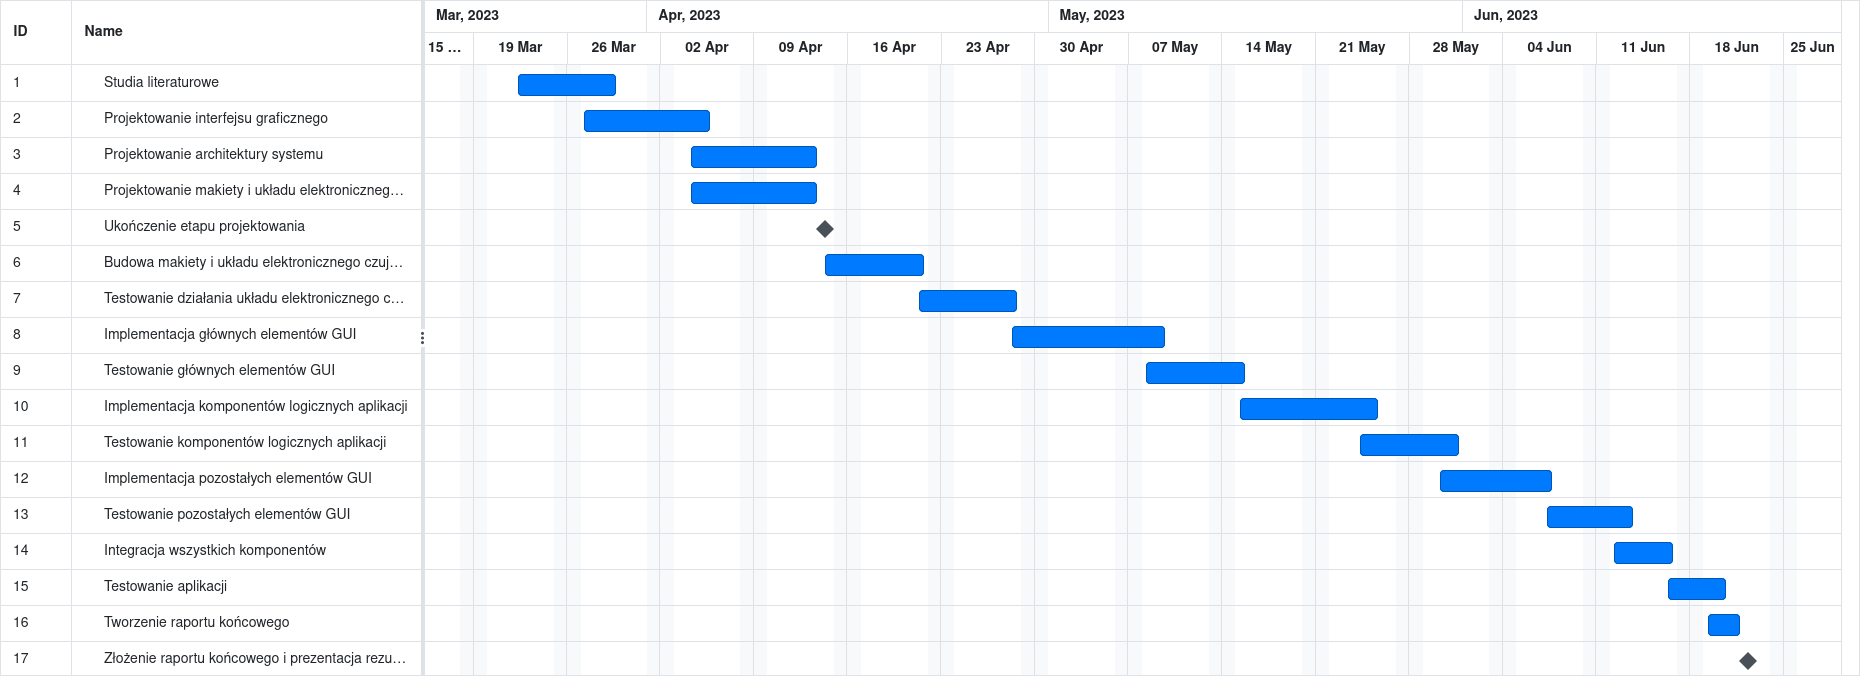
\includegraphics[width = \textheight, angle = 270]{obrazy/wsd_gantt.png}
    \caption{Wykres gantta}
    \label{fig: gantt}
\end{figure}


\end{document}
